\documentclass{article}
\setlength{\parindent}{0pt} % Remove indent at new paragraphs
\setcounter{secnumdepth}{0}	% Remove section numbering at certain depth
\usepackage[round,sort]{natbib}
\usepackage{fixltx2e}
\usepackage{graphicx}	% For external pictures
\usepackage{float}
\usepackage{subfig}	% Add subfigures within figures
\usepackage{verbatim}
\usepackage[colorlinks=true,linkcolor=blue,citecolor=blue,urlcolor=blue]{hyperref}
\usepackage{amssymb,amsbsy,amsmath}
\usepackage{epsfig}
\usepackage[left=3cm,top=3cm,bottom=3.5cm,right=3cm]{geometry} % For easy document margins
\usepackage{fancyhdr} % For customization of header/footer
\numberwithin{equation}{section} % Equation numbers relative to sections

% ---------------------------------------------------------------------------------------------------------------------------------------

% \VignetteIndexEntry{ggenealogy: Visualization tools for genealogical data}
%\VignetteDepends{quantreg,nnet}
%\VignettePackage{ggenealogy}
%\documentclass{amsart}
\newcommand{\code}[1]{{\texttt{#1}}}
\newcommand{\pkg}[1]{{\texttt{#1}}}
\newcommand{\class}[1]{{\textit{#1}}}
\newcommand{\R}{{\normalfont\textsf{R }}{}}

\usepackage{Sweave}
\begin{document}
\Sconcordance{concordance:ggenealogy.tex:ggenealogy.Rnw:%
1 27 1 1 0 23 1 1 4 26 1 1 2 4 0 1 2 2 1 1 2 4 0 1 2 2 1 1 2 4 0 1 2 2 %
1 1 2 1 0 2 1 3 0 1 2 4 1 1 2 1 0 1 1 11 0 1 1 5 0 1 1 11 0 1 2 4 1 1 2 %
4 0 1 2 4 1 1 2 1 0 1 1 6 0 1 2 5 1 4 0 1 3 14 1 1 2 6 0 1 1 6 0 1 2 4 %
1 1 2 6 0 1 1 6 0 1 2 4 1 1 2 6 0 1 1 6 0 1 2 4 1 1 2 6 0 1 1 5 0 1 1 6 %
0 1 2 4 1 1 2 6 0 1 1 8 0 1 2 6 1 1 2 9 0 1 2 4 1 1 2 33 0 1 1 6 0 1 2 %
4 1 1 2 19 0 1 2 4 1 1 2 35 0 1 2 6 1 1 2 6 0 1 1 6 0 1 2 8 1 1 2 26 0 %
1 2 4 1 1 2 1 0 1 1 11 0 1 1 6 0 1 2 2 1 1 2 1 0 1 1 6 0 1 1 6 0 1 2 10 %
1 1 2 4 0 1 2 3 1 1 -5 1 9 14 1 1 2 4 0 1 2 3 1 1 -5 1 9 14 1 1 2 11 0 %
1 2 4 1 1 2 1 0 1 1 6 0 1 2 2 1 1 2 7 0 1 2 4 1 1 2 4 0 1 2 2 1 1 2 4 0 %
1 2 3 1 1 -5 1 9 10 1 1 2 1 0 1 1 3 0 1 2 3 1 1 -5 1 9 6 1 1 2 1 0 1 1 %
3 0 2 2 1 0 1 1 3 0 1 2 3 1 1 -5 1 9 10 1 1 2 4 0 1 2 3 1 1 -5 1 9 18 1 %
1 2 4 0 1 2 3 1 1 -5 1 9 12 1 1 2 1 0 2 1 3 0 1 2 3 1 1 -5 1 9 6 1 1 2 %
7 0 1 2 4 1 1 2 1 0 1 1 3 0 1 2 3 1 1 -5 1 9 15 1}


% <<label=R options,echo=FALSE>>=
% options(width = 60)
% options(SweaveHooks = list(fig = function() par(mar=c(3,3,1,0.5),mgp = c(2,1,0))))
% @

%\SweaveOpts{prefix.string=fig,include=F,keep.source=T,eps=FALSE}

% <<echo=false>>=
% options(continue="  ")
% @
% %@% TO ELIMINATE THE "+" IN CONSECUTIVE SCRIPT LINES

\title{Vignette: Grammar of graphics of genealogy (ggenealogy)}
\author{Lindsay Rutter, Susan Vanderplas, Di Cook}
\date{\pkg{ggenealogy} version 0.1 , 2015-02-24 }
\maketitle

\tableofcontents
\setcounter{footnote}{1} \footnotetext{This \LaTeX\ vignette document is created using the \R function \code{Sweave}) on the \R package \pkg{ggenealogy}. It is automatically downloaded with the package and can be accessed with the \R command \code{vignette("ggenealogy")}.}  \newpage
\setlength{\parskip}{4pt} % Inter-paragraph spacing


\section{Summary}

\textbf{Description} 

The \pkg{ggenealogy} package provides tools to examine genealogical data, generating basic statistics on their graphical structures using parent and child connections, and displaying the results. The genealogy can be drawn in relation to additional variables, such as development year, and the shortest path distances between genetic lines can be determined and displayed. Production of pairwise distance matrices and phylogenetic diagrams constrained by generation count are also available in the visualization toolkit. This vignette is intended to walk readers through the different methods available in the \pkg{ggenealogy} package.

\bigskip

\textbf{Caution}

\texttt{igraph} must be used with version >= 0.7.1

\section{Introduction}

\subsection{Installation}

\R is a open source software project for statistical computing, and can be freely downloaded from the Comprehensive R Archive Network (CRAN) website. The link to contributed documentation on the CRAN website offers practical resources for an introduction to \R, in several languages. After downloading and installing \R, the installation of additional packages is straightforward. To install the \pkg{ggenealogy} package from \R, use the command:

\vspace{2mm}
\noindent
\texttt{> install.packages("ggenealogy")}

\vspace{2mm}
\noindent
The \pkg{ggenealogy} package should now be successfully installed. Next, to render it accessible to the current \R session, simply type:

\begin{Schunk}
\begin{Sinput}
> library(ggenealogy)
\end{Sinput}
\end{Schunk}

To access help pages with example syntax and documentation for the available functions of the \pkg{ggenealogy} package, please type:

\begin{Schunk}
\begin{Sinput}
> help(package="ggenealogy")
\end{Sinput}
\end{Schunk}

To access more detailed information about a specific function in the \pkg{ggenealogy} package, use the following help command on that function, such as:

\begin{Schunk}
\begin{Sinput}
> help(getChild)
\end{Sinput}
\end{Schunk}

The above command will return the help file for the \texttt{getChild} function. The help file often includes freestanding example syntax to illustrate how function commands are executed. In the case of the \texttt{getChild} function, the example syntax is the following three lines, which can be pasted directly into an \R session.

\begin{Schunk}
\begin{Sinput}
> data(sbGeneal)
> getChild("Tokyo", sbGeneal)
> getChild("Essex", sbGeneal)
\end{Sinput}
\end{Schunk}

\subsection{Preprocessing pipeline}

In the \pkg{ggenealogy} package, there is an example dataset containing genealogical information on soybean varieties called \texttt{sbGeneal.rda}. It may be helpful to load that example file so that you can follow along with the commands and options introduced in this vignette. To ensure that you have uploaded the correct, raw \texttt{sbGeneal.rda} file, you can observe the first six lines of the file, and determine its dimension and structure:

\begin{Schunk}
\begin{Sinput}
> data(sbGeneal)
> head(sbGeneal)
\end{Sinput}
\begin{Soutput}
          child year yield year.imputed    parent
1         5601T 1981    NA         TRUE Hutcheson
2         Adams 1948  2734        FALSE  Dunfield
3          A.K. 1910    NA         TRUE      <NA>
4 A.K. (Harrow) 1912  2665        FALSE      A.K.
5        Altona 1968    NA        FALSE  Flambeau
6         Amcor 1979  2981        FALSE  Amsoy 71
\end{Soutput}
\begin{Sinput}
> dim(sbGeneal)
\end{Sinput}
\begin{Soutput}
[1] 412   5
\end{Soutput}
\begin{Sinput}
> str(sbGeneal)
\end{Sinput}
\begin{Soutput}
'data.frame':	412 obs. of  5 variables:
 $ child       : chr  "5601T" "Adams" "A.K." "A.K. (Harrow)" ...
 $ year        : num  1981 1948 1910 1912 1968 ...
 $ yield       : int  NA 2734 NA 2665 NA 2981 2887 2817 NA NA ...
 $ year.imputed: logi  TRUE FALSE TRUE FALSE FALSE FALSE ...
 $ parent      : chr  "Hutcheson" "Dunfield" NA "A.K." ...
\end{Soutput}
\end{Schunk}

We see that the \texttt{sbGeneal} data file is a data frame structure with 412 rows (observations) and 5 columns (variables). Each row contains a \texttt{child} node character label and \texttt{parent} node character label. Each row also contains a numeric value corresponding to the \texttt{year} the child node was introduced, an integer value of the protein \texttt{yield} of the child node, and a logical value \texttt{year.imputed}, which indicates whether or not the year of introduction of the child node was imputed.

Now that the \texttt{sbGeneal} file has been loaded as a data frame, it must next be converted into a graph object using the \texttt{dfToIG()} function. The \texttt{dfToIG()} function requires a data frame as input, and that data frame should be structured such that each row represents an edge with a child and parent relationship. For more information, try using the help command on the function:

\begin{Schunk}
\begin{Sinput}
> help(dfToIG)
\end{Sinput}
\end{Schunk}

We see that the function takes optional parameter arguments, such as \texttt{vertexinfo} (a list of columns of the data frame which provide information for the starting ``child" vertex, or a separate data frame containing information for each vertex with the first column as the vertex name), \texttt{edgeweights} (a column that contains edge values, with a default value of unity), and \texttt{isDirected} (a boolean value that describes whether the graph is directed (true) or undirected (false); the default is false).

In this example, we want to produce an undirected graph object that contains all edge weight values of one, because our goal is to set an edge value of unity for every pair of vertices (individuals) that are related as parent and child. The \texttt{dfToIG()} function uses the software \texttt{igraph} to convert the data frame into a graph object. For clarity, we will assign the outputted graph object the name \texttt{ig} (for \texttt{igraph} object), and then examine its class type:

\begin{Schunk}
\begin{Sinput}
> ig <- dfToIG(sbGeneal)
> class(ig)
\end{Sinput}
\begin{Soutput}
[1] "igraph"
\end{Soutput}
\end{Schunk}

Above, we confirmed that the \texttt{ig} object is of class type \texttt{igraph}.

We can add the other data we have about each of the nodes in \texttt{ig} in several ways. As we saw earlier, each row of the \texttt{sbGeneal} dataset contains information about each child. To append that data to the \texttt{ig} object, we can use the same command as before, but specify the \texttt{vertexinfo} parameter as follows: 

\begin{Schunk}
\begin{Sinput}
> #ig <- dfToIG(sbGeneal, vertexinfo=c("year", "yield", "year.imputed"))
\end{Sinput}
\end{Schunk}

If we have separate data sets with node information, we can use that instead. For the example dataset, we must first obtain the node information: 

The \texttt{ig} object is used in many of the other functions included with this package. 

\section{General (non-plotting) methods of genealogical data}

The \pkg{ggenealogy} package offers several functions that you can use to obtain information without producing plots. Below is a brief introduction of some of those functions.

\subsection{Functions for individual vertices}

The \pkg{ggenealogy} package offers several functions that you can use to obtain information for individual vertices.

First, the function \texttt{isParent()} can return a logical variable to indicate whether or not the second variety is a parent of the first variety.

\begin{Schunk}
\begin{Sinput}
> isParent("Young","Essex",sbGeneal)
\end{Sinput}
\begin{Soutput}
[1] TRUE
\end{Soutput}
\begin{Sinput}
> isParent("Essex","Young",sbGeneal)
\end{Sinput}
\begin{Soutput}
[1] FALSE
\end{Soutput}
\end{Schunk}

We see that ``Essex" is a parent of ``Young".

Similarly, the function \texttt{isChild()} can return a logical variable to indicate whether or not the first variety is a child of the second variety.

\begin{Schunk}
\begin{Sinput}
> isChild("Young","Essex",sbGeneal)
\end{Sinput}
\begin{Soutput}
[1] TRUE
\end{Soutput}
\begin{Sinput}
> isChild("Essex","Young",sbGeneal)
\end{Sinput}
\begin{Soutput}
[1] FALSE
\end{Soutput}
\end{Schunk}

We see that, as expected, ``Young" is a child of ``Essex".

It is also possible to derive the year of a given variety using the \texttt{getYear()} function:

\begin{Schunk}
\begin{Sinput}
> getYear("Young",sbGeneal)
\end{Sinput}
\begin{Soutput}
[1] 1968
\end{Soutput}
\begin{Sinput}
> getYear("Essex",sbGeneal)
\end{Sinput}
\begin{Soutput}
[1] 1962
\end{Soutput}
\end{Schunk}

Fortunately, the returned year values are consistent, as the ``Young" variety (1968) is a child to the ``Essex" variety (1962) by an age difference of six years.

In some cases, you may wish to obtain a complete list of all the parents of a given variety. This can be achieved using the \texttt{getParent()} function:

\begin{Schunk}
\begin{Sinput}
> getParent("Young",sbGeneal)
\end{Sinput}
\begin{Soutput}
[1] "Davis" "Essex"
\end{Soutput}
\begin{Sinput}
> getParent("Tokyo",sbGeneal)
\end{Sinput}
\begin{Soutput}
character(0)
\end{Soutput}
\begin{Sinput}
> getYear("Tokyo", sbGeneal)
\end{Sinput}
\begin{Soutput}
[1] 1907
\end{Soutput}
\end{Schunk}

We learn from this that ``Essex" is not the only parent of ``Young"; it also has a parent ``Davis". We also see that ``Tokyo" does not have any documented parents in this dataset, and has an older year of introduction (1907) than other varieties we have examined thusfar.

Likewise, in other cases, you may wish to obtain a complete list of all the children of a given variety. This can be achieved using the \texttt{getChild()} function:

\begin{Schunk}
\begin{Sinput}
> getChild("Tokyo",sbGeneal)
\end{Sinput}
\begin{Soutput}
[1] "Ogden"    "Volstate"
\end{Soutput}
\begin{Sinput}
> getChild("Ogden",sbGeneal)
\end{Sinput}
\begin{Soutput}
 [1] "C1069"          "C1079"          "D51-2427"       "D55-4090"      
 [5] "D55-4159"       "D55-4168"       "Kent"           "N44-92"        
 [9] "N45-745"        "N48-1101"       "Ogden x CNS"    "Ralsoy x Ogden"
\end{Soutput}
\end{Schunk}

We find that even though the ``Tokyo" variety is a grandparent of the dataset, it only has two children, ``Ogden" and ``Volstate". However, one of its children, ``Ogden", produced twelve children.

If we want to obtain a list that contains more than just one generation past or previous to a given variety, then we can use the \texttt{getAncestors()} and \texttt{getDescendants()} functions, where we specify the number of generations we wish to view. This will return a data frame to us with the labels of each ancestor or descendant, along with the number of generations each one is from the given variety.

If we only look at one generation of ancestors of the ``Young" variety, we should see the same information we did earlier when we used the \texttt{getParent()} function of the Young variety:

\begin{Schunk}
\begin{Sinput}
> getAncestors("Young",sbGeneal,1)
\end{Sinput}
\begin{Soutput}
  label gen
2 Davis   1
1 Essex   1
\end{Soutput}
\end{Schunk}

Indeed, we consistently see that the ``Young" variety has only two ancestors within one generation, ``Davis" and ``Essex".

However, if we view the first five generations of ancestors of the ``Young" variety, we can view four more generations of ancestors past simply the parents:

\begin{Schunk}
\begin{Sinput}
> getAncestors("Young",sbGeneal,5)
\end{Sinput}
\begin{Soutput}
                     label gen
27                   Davis   1
26                   Essex   1
25          Ralsoy x Ogden   2
24 Roanoke x (Ogden x CNS)   2
23                     Lee   2
22                S55-7075   2
21                   Ogden   3
20                  Ralsoy   3
19             Ogden x CNS   3
17                     CNS   3
18                 Roanoke   3
16                   S 100   3
15                N48-1248   3
14                   Perry   3
10                   Ogden   4
13                PI 54610   4
12                   Tokyo   4
11                     CNS   4
9                  Clemson   4
6                  Roanoke   4
8                   Illini   4
7  N45-745 x (Ogden x CNS)   4
4                 PI 54610   5
3                    Tokyo   5
1              Ogden x CNS   5
5                  Clemson   5
2                     A.K.   5
\end{Soutput}
\begin{Sinput}
> dim(getAncestors("Young",sbGeneal,5))
\end{Sinput}
\begin{Soutput}
[1] 27  2
\end{Soutput}
\end{Schunk}

In the second line of code above, we determined the dimensions of the returned data frame, and see that there are 27 ancestors within the first five ancestral generations of the ``Young" variety.

Similarly, if we only look at the first generation of descendants of the ``Ogden" variety, we should see the same information as we did earlier when we used the \texttt{getChild()} function on the ``Ogden" variety:

\begin{Schunk}
\begin{Sinput}
> getDescendants("Ogden",sbGeneal,1)
\end{Sinput}
\begin{Soutput}
            label gen
12          C1069   1
11          C1079   1
10       D51-2427   1
9        D55-4090   1
8        D55-4159   1
7        D55-4168   1
6            Kent   1
5          N44-92   1
4         N45-745   1
3        N48-1101   1
2     Ogden x CNS   1
1  Ralsoy x Ogden   1
\end{Soutput}
\end{Schunk}

Indeed, we see again that ``Ogden" has 12 children. 

However, if we want to view not only the children, but also the grandchildren, of the ``Ogden" variety, then we can use this function, only now specifying two generations of descendants:

\begin{Schunk}
\begin{Sinput}
> getDescendants("Ogden",sbGeneal,2)
\end{Sinput}
\begin{Soutput}
                     label gen
28                   C1069   1
27                   C1079   1
26                D51-2427   1
25                D55-4090   1
24                D55-4159   1
23                D55-4168   1
22                    Kent   1
21                  N44-92   1
20                 N45-745   1
19                N48-1101   1
18             Ogden x CNS   1
17          Ralsoy x Ogden   1
16                Columbus   2
15                  Cutler   2
14                  C1266R   2
13                  Semmes   2
11                D60-7965   2
12                D60-7965   2
10                D59-9289   2
9                   Beeson   2
8                  Calland   2
7                     Hood   2
6                 N48-1867   2
5                  D52-810   2
4  N45-745 x (Ogden x CNS)   2
3                  R54-168   2
2  Roanoke x (Ogden x CNS)   2
1                    Davis   2
\end{Soutput}
\end{Schunk}

We see that variety ``Ogden" has 16 grandchildren from its 12 children.

\subsection{Functions for pairs of vertices}

Say you have a pair of vertices, and you wish to determine the degree of the shortest path between them, where edges represent parent-child relationships. You can accomplish that with the \texttt{getDegree()} function.

\begin{Schunk}
\begin{Sinput}
> getDegree("Tokyo", "Ogden", ig, sbGeneal)
\end{Sinput}
\begin{Soutput}
[1] 1
\end{Soutput}
\begin{Sinput}
> getDegree("Tokyo", "Holladay", ig, sbGeneal)
\end{Sinput}
\begin{Soutput}
[1] 7
\end{Soutput}
\end{Schunk}

As expected, the shortest path between the ``Tokyo" and ``Ogden" varieties has a value of one, as we already determined that they have a direct parent-child relationship. However, the shortest path between ``Tokyo" and one of its descendants, ``Holladay", has a much higher degree of seven.

Note that degree calculations in this case are not limited to one linear string of parent-child relationships; cousins and siblings and products thereof will also have computable degrees via nonlinear strings of parent-child relationships.

\subsection{Functions for the full genealogical structure}

There are many parameters about the full genealogical structure that you may wish to know that cannot easily be obtained through images and tables. The function \texttt{getBasicStatistics()} will return graph theoretical measurements of the full genealogy. For instance, is the full genealogy connected? If not, how many separated components does it contain? In addition to these parameters, the \texttt{getBasicStatistics()} function will also return the number of nodes, the number of edges, the average path length, the graph diameter, among others:

\begin{Schunk}
\begin{Sinput}
> getBasicStatistics(ig)
\end{Sinput}
\begin{Soutput}
$isConnected
[1] FALSE

$numComponents
[1] 11

$avePathLength
[1] 5.333746

$graphDiameter
[1] 13

$numNodes
[1] 230

$numEdges
[1] 340

$logN
[1] 5.438079
\end{Soutput}
\end{Schunk}

In this case, we learn that our full genealogical structure is actually not all connected by parent-child edges, and that instead, it is composed of 11 separate components. We see that the average path length of the full genealogy is 5.333, that the graph diameter is 13, and that the logN value is 5.438. We also see that the number of nodes in the full genealogy is 230, and the number of edges in the full genealogy is 340.

But can we view a list of these nodes and edges? To do so, we can call the \texttt{getNodes()} and \texttt{getEdges()} commands to obtain lists of all the unique nodes and edges in the full genealogical structure. Here, we obtain a list of the 340 edges (with each row containing the names of the two connected vertices, and an edge weight, if existent). We will simply view the first six rows of the object, and determine the number of edges by counting the number of rows (340):

\begin{Schunk}
\begin{Sinput}
> eList = getEdges(ig, sbGeneal)
> head(eList)
\end{Sinput}
\begin{Soutput}
     child           parent     
[1,] "5601T"         "Hutcheson"
[2,] "Adams"         "Dunfield" 
[3,] "A.K. (Harrow)" "A.K."     
[4,] "Altona"        "Flambeau" 
[5,] "Amcor"         "Amsoy 71" 
[6,] "Amsoy"         "Adams"    
\end{Soutput}
\begin{Sinput}
> dim(eList)
\end{Sinput}
\begin{Soutput}
[1] 340   2
\end{Soutput}
\end{Schunk}

We then obtain a list of the 230 nodes. Again, we only view the first six rows of the object, and determine the number of nodes by counting the number of rows (230).

\begin{Schunk}
\begin{Sinput}
> nList = getNodes(sbGeneal)
> head(nList)
\end{Sinput}
\begin{Soutput}
[1] "5601T"         "Adams"         "A.K."          "A.K. (Harrow)"
[5] "Altona"        "Amcor"        
\end{Soutput}
\begin{Sinput}
> length(nList)
\end{Sinput}
\begin{Soutput}
[1] 230
\end{Soutput}
\end{Schunk}

\section{Plotting methods of genealogical data}

Until this point, the vignette has introduced functions that return lists, data frames, and statistics about the genealogical dataset. However, the \pkg{ggenealogy} package also contains visualization tools for genealogical datasets. Access to various types of visual plots and diagrams of the lineage can allow genealogical researchers to more efficiently and accurately explore an otherwise complicated data structure. Below, we introduce functions in \pkg{ggenealogy} that produce visual outputs of the dataset.

\subsection{Plotting the ancestors and descendants of a vertex}

One visualization tool, \texttt{plotAncDes()}, allows the user to view the ancestors and descendants of a given variety. The inputted variety is highlighted in the center of the plot, ancestors are displayed to the left of the center, and descendants are displayed to the right of the center. The further left or right from the center, the larger the number of generations that particular ancestor/descendant is from the inputted and centered variety.

As such, this plotting command does not provide visual information about specific years associated with each related variety (as is done in some of the visualization tools introduced later), but it does group all varieties from each generation group onto the same position of the horizontal axis. Here, we specify that we want to plot 3 ancestor generations and 5 descendant generations of the variety ``Lee":

\begin{Schunk}
\begin{Sinput}
> plotAncDes("Lee", sbGeneal, 3, 5)
\end{Sinput}
\end{Schunk}

\setkeys{Gin}{width=6in, height=6in}
\begin{figure} 
  \begin{center} 
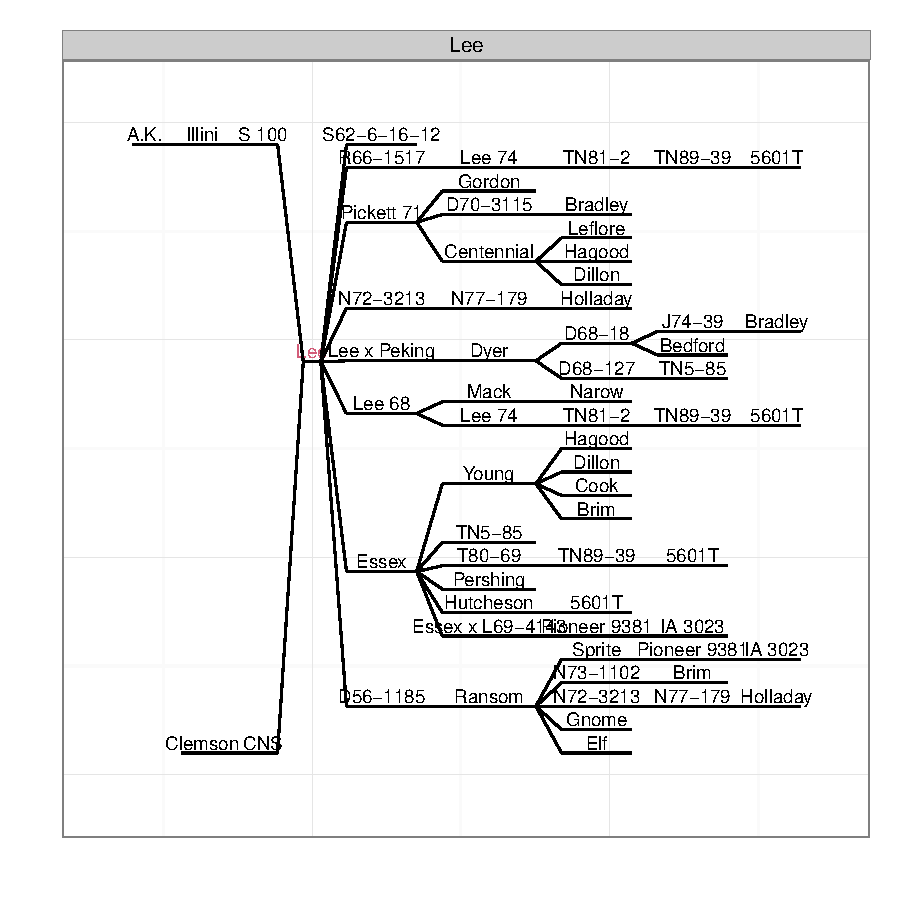
\includegraphics{ggenealogy-plotAncDes1}
\end{center} 
\caption{Ancestors and Descendants of tree.}
\label{fig:plotAncDes1}
\end{figure}

We immediately see that this visual representation of the ancestors and descendants of a given variety can often provide enhanced readability compared to the list output provided in the previous similar functions, \texttt{getAncestors()} and \texttt{getDescendants()}.

We also see now that some node labels are repeated. For instance, the ``5601T" variety appears twice, once as a grandchild (second generation descendant) of ``Essex", and once as a great-granchild (third generation descendant) of ``Essex". This is because there are two separate parent-child pathways between ``Essex" and ``5601T", one pathway with only one node (``Hutchson") between them, and one pathway with two nodes (``T80-69" and ``TN89-39") between them.

However, in this visual tool, we are constraining the horizontal axis to generation count. Without allowing nodes to repeat, this data information cannot be clearly and succinctly presented. Most graph visualization software that genealogists might use to view their datasets do not allow for repeated nodes, as per the definition of a graph. Hence, the \texttt{plotAncDes()} function is one of the more unique visual tools of the \pkg{ggenealogy} package.

It should be noted that the \texttt{plotAncDes()} function, by default, highlights the centered variety label in pink. However, the user can alter this color, as we will show below. Furthermore, the user can specify additional grammar of graphics plotting tools (from the \texttt{ggplot2} package) to tailor the output of the \texttt{plotAncDes()} function.

For example, we will now change the color of the center variety label \texttt{vColor} to be highlighted in blue. Also, we will add a horizontal axis label called ``Generation index", using the \texttt{ggplot2} syntax. Note that this time we do not specify the generational count for ancestors and descendants, and so the default value of three generations is applied for both cases. Remember, to determine such default values, as well as all possible function parameters, simply run the help command on the function of interest, as in help(plotAncDes).

\begin{Schunk}
\begin{Sinput}
> plotAncDes("Tokyo", sbGeneal, vColor = "blue") + ggplot2::labs(x="Generation index",y="")
\end{Sinput}
\end{Schunk}

\setkeys{Gin}{width=6in, height=6in}
\begin{figure} 
  \begin{center} 
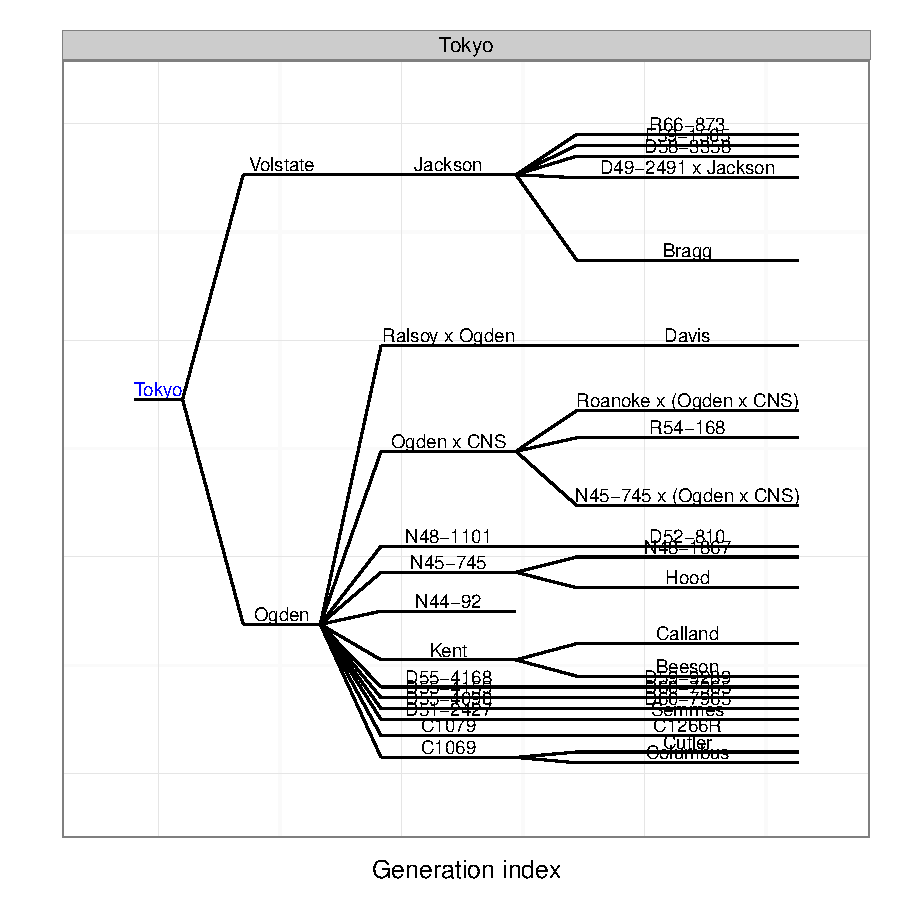
\includegraphics{ggenealogy-plotAncDes2}
\end{center} 
\caption{Ancestors and Descendants of tree.}
\label{fig:plotAncDes2}
\end{figure}

We verify immediately that the ``Tokyo" variety does not have any ancestors in this dataset, an observation consistent with what we discovered earlier. We also see the ``Tokyo" variety only has two children, but has many more grandchildren, and great-grand children.

\subsection{Plotting the shortest path between two vertices}

As this data set deals with soy bean lineages, it may be useful for agronomists to track how two varieties are related to each other via parent-child relationships. Then, any dramatic changes in protein yield, SNP varieties, and other measures of interest between the two varieties can be tracked across their genetic timeline, and pinpointed to certain varieties within their historical lineage.

The \pkg{ggenealogy} software allows users to select two varieties of interest, and determine the shortest pathway of parent-child relationships between them, using the \texttt{getPath()} function. This will return a list path object that contains the variety names and their years in the path. The returned path object can then be plotted using the \texttt{plotPath()} function:

The \texttt{getPath()} function determines the shortest path between the two inputted vertices, and takes into account whether or not the graph is directed with the parameter \texttt{isDirected}, which defaults to false. The \texttt{getPath()} function will check both directions and return the path if it exists:

\begin{Schunk}
\begin{Sinput}
> getPath("Brim","Bedford", ig, sbGeneal, isDirected=FALSE)
\end{Sinput}
\begin{Soutput}
$pathVertices
[1] "Brim"    "Young"   "Essex"   "T80-69"  "J74-40"  "Forrest" "Bedford"

$yearVertices
[1] "1977" "1968" "1962" "1975" "1975" "1973" "1978"
\end{Soutput}
\end{Schunk}

We see that there is a path between ``Brim" and ``Bedford" varieties, with five varieties separating them. We are not considering direction, however, because the \texttt{ig} object is undirected.

However, to demonstrate the importance of direction, we will recompute the path where the direction matters. We first produce a directed \texttt{igraph} object \texttt{dirIG}, and then try to determine the path between the same two vertices, ``Brim" and ``Bedford".

\begin{Schunk}
\begin{Sinput}
> dirIG = dfToIG(sbGeneal, isDirected = TRUE)
> getPath("Brim", "Bedford", dirIG, sbGeneal, isDirected = TRUE)
\end{Sinput}
\begin{Soutput}
list()
\end{Soutput}
\end{Schunk}

Now that we are considering the direction, we are only considering paths where each edge represents a parent-child relationship in the same direction as the one before it. We now receive an empty return list with a warning that there is no path between those two vertices. We  next try to reverse the input order of the vertices, as shown below, but we will receive the same empty return list and warning:

\begin{Schunk}
\begin{Sinput}
> getPath("Bedford", "Brim", dirIG, sbGeneal, isDirected=TRUE)
\end{Sinput}
\begin{Soutput}
list()
\end{Soutput}
\end{Schunk}

We can derive from the empty list returned in the last two commands that the varieties ``Brim" and ``Bedford" are not connected by a linear sequence of parent-child relationships. Rather, the path between them branches at some point, involving siblings and/or cousins.

Hence, unless you are working with a dataset that must be analyzed as a directed graph, it is best to use the \texttt{getPath()} function with the default third parameter indicating lack of direction, and to use an \texttt{igraph} object without direction, such as \texttt{ig}. We do just that, and save the path between these two varieties to a variable called \texttt{path}:

\begin{Schunk}
\begin{Sinput}
> path = getPath("Bedford","Brim", ig, sbGeneal, isDirected=FALSE)
\end{Sinput}
\end{Schunk}

Now that we have a non-empty \texttt{path} object that consists of two lists (for variety names and years), we can plot the relationship between the two using the \texttt{plotPath()} function.

\begin{Schunk}
\begin{Sinput}
> plotPath(path)
\end{Sinput}
\end{Schunk}

\setkeys{Gin}{width=6in, height=6in}
\begin{figure} 
  \begin{center} 
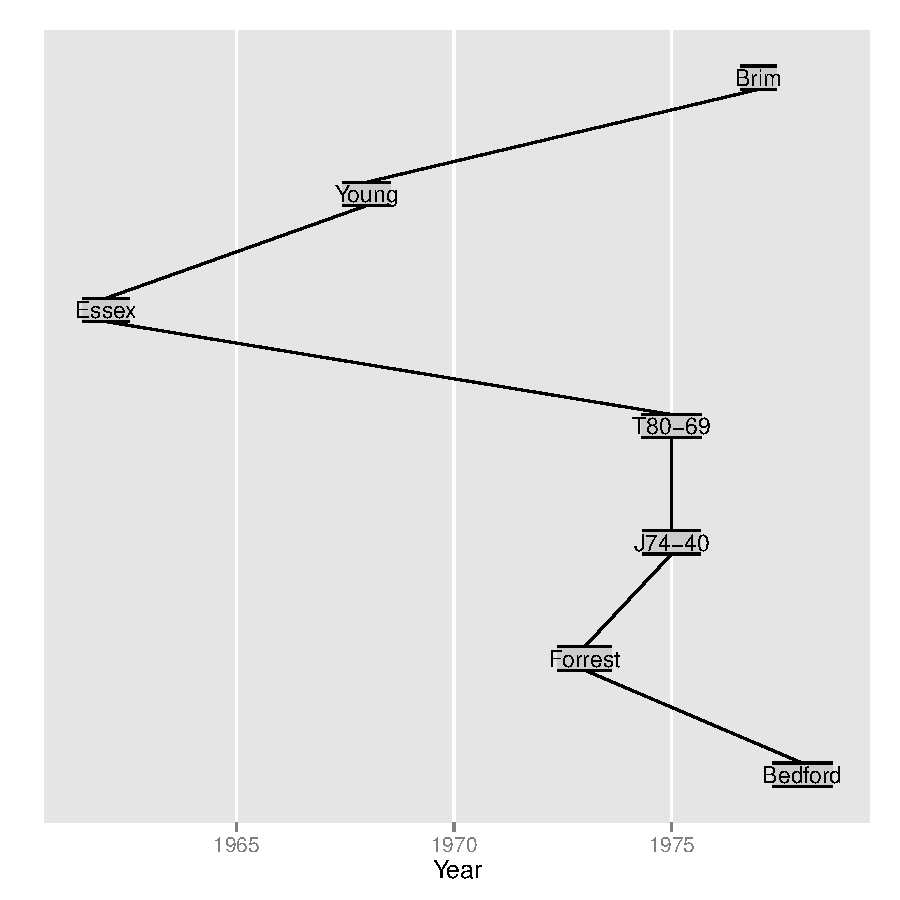
\includegraphics{ggenealogy-plotPath1}
\end{center} 
\caption{Ancestors and Descendants of tree.}
\label{fig:plotPath1}
\end{figure}

This produces a neat visual that informs us of all the varieties involved in the shortest path between ``Brim" and ``Bedford". In this plot, the years of all varieties involved in the path are indicated on the horizontal axis, while the vertical axis has no meaning other than to simply to display the labels evenly spaced vertically. 

Although a call to the \pkg{ggenealogy} function \texttt{getYear()} indicates that ``Bedford" was developed in 1978 and ``Brim" in 1977, we quickly determine from the plot that ``Brim" is not a parent, grandparent, nor any great grandparent of ``Bedford". Instead, we see that these two varieties are not related through a unidirectional parent-child lineage, but have a cousin-like relationship. The oldest common ancestor between ``Bedford" and ``Brim" is the variety ``Essex", which was developed in 1962.

However, there are other cases of pairs of varieties that are connected by a linear, unidirectional combination of parent-child relationships, as we see below:

\begin{Schunk}
\begin{Sinput}
> path = getPath("Narow", "Tokyo", ig, sbGeneal, isDirected=FALSE)
> plotPath(path)
\end{Sinput}
\end{Schunk}

\setkeys{Gin}{width=6in, height=6in}
\begin{figure} 
  \begin{center} 
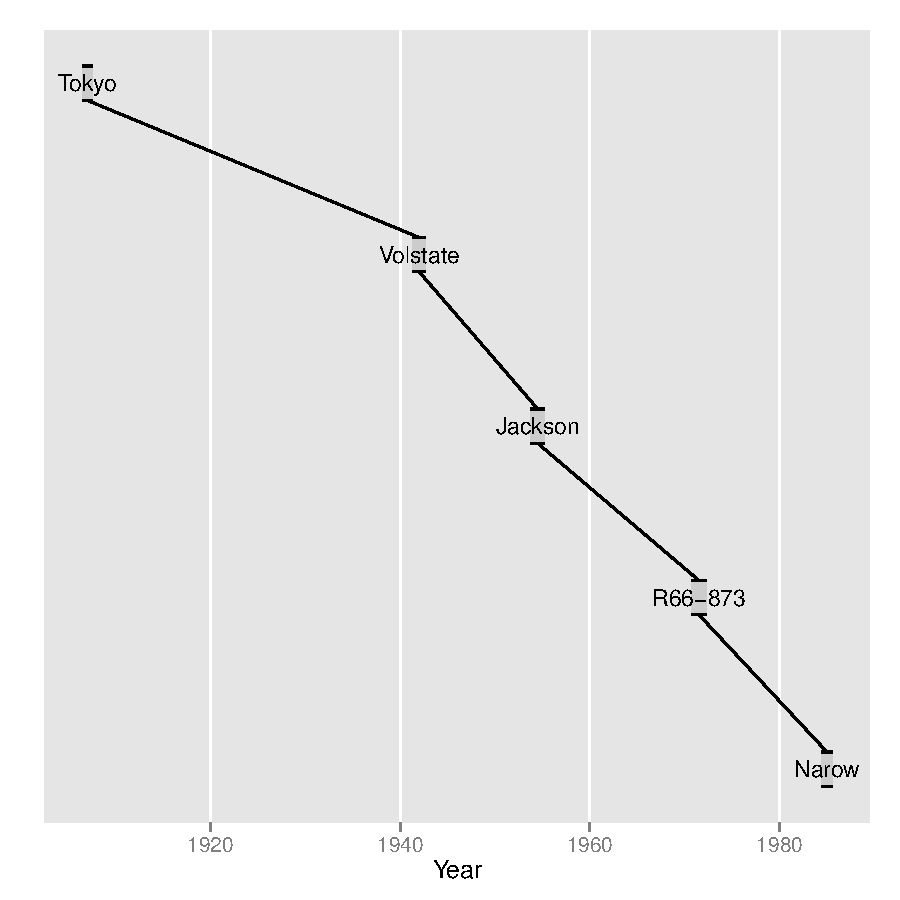
\includegraphics{ggenealogy-plotPath2}
\end{center} 
\caption{Ancestors and Descendants of tree.}
\label{fig:plotPath2}
\end{figure}

Here, we see that the variety ``Tokyo" is an ancestor of ``Narow" via four linear parent-child relationships. Because of this, we can still view the pathway, even when we use an \texttt{igraph} object \texttt{dirIG} that is directed, and set the boolean \texttt{isDirected} variable to true. Either ordering of the two varieties will produce the exact same result:

\begin{Schunk}
\begin{Sinput}
> path = getPath("Narow", "Tokyo", dirIG, sbGeneal, isDirected=TRUE)
> plotPath(path)
\end{Sinput}
\end{Schunk}

\begin{Schunk}
\begin{Sinput}
> path = getPath("Tokyo", "Narow", dirIG, sbGeneal, isDirected=TRUE)
> plotPath(path)
\end{Sinput}
\end{Schunk}

\setkeys{Gin}{width=6in, height=6in}
\begin{figure} 
  \begin{center} 
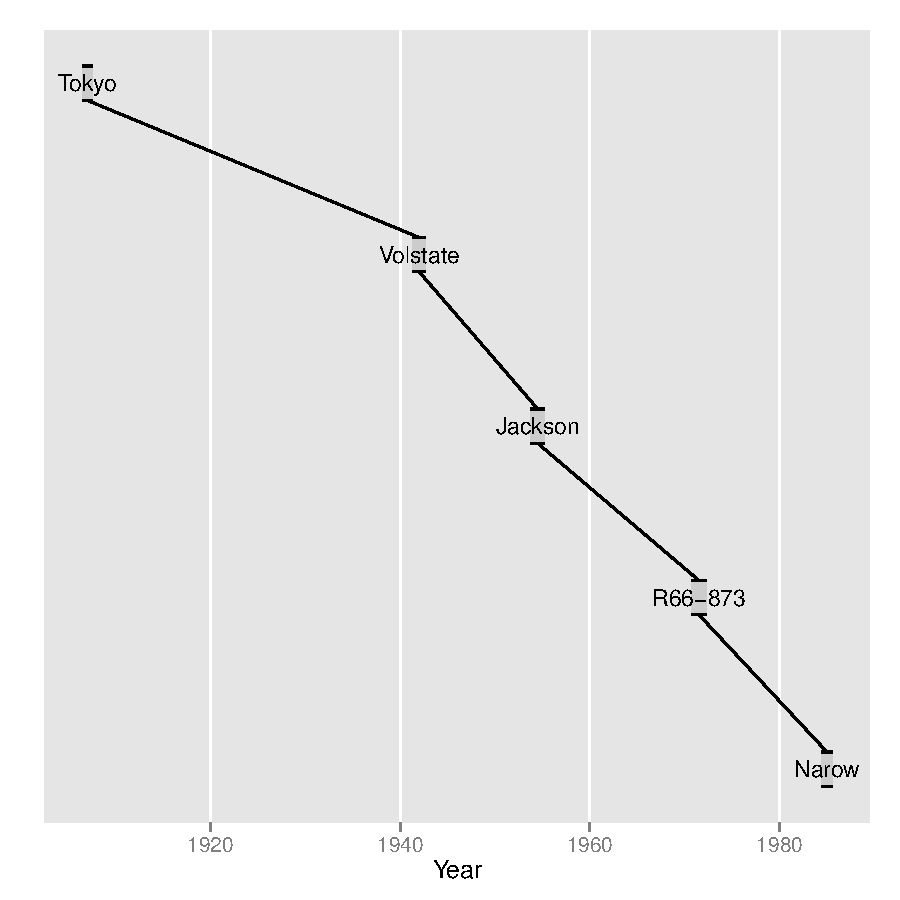
\includegraphics{ggenealogy-plotPath3}
\end{center} 
\caption{Ancestors and Descendants of tree.}
\label{fig:plotPath3}
\end{figure}

\subsection{Plotting shortest paths superimposed on full genealogical structure}

Now that we can create and plot path objects, we may wish to know how those paths are positioned in comparison to the genealogical lineage of the entire data structure. For instance, of the documented soybean cultivar lineage varieties, where does the shortest path between two varieties of interest exist? Are these two varieties comparatively older compared to the overall data structure? Are they newer? Or, do they span the entire structure, and represent two extreme ends of documented time points?

There is a function available in the \pkg{ggenealogy} package, \texttt{plotPathOnAll()}, that allows users to quickly visualize their path of interest superimposed over all varieties and edges present in the whole data structure. Here we will produce a plot of the previously-determined shortest path between varieties Tokyo and Narow across the entire dataset:

\begin{Schunk}
\begin{Sinput}
> plotPathOnAll(path, sbGeneal, ig, binVector = 1:3)
\end{Sinput}
\end{Schunk}

\setkeys{Gin}{width=6in, height=6in}
\begin{figure} 
  \begin{center} 
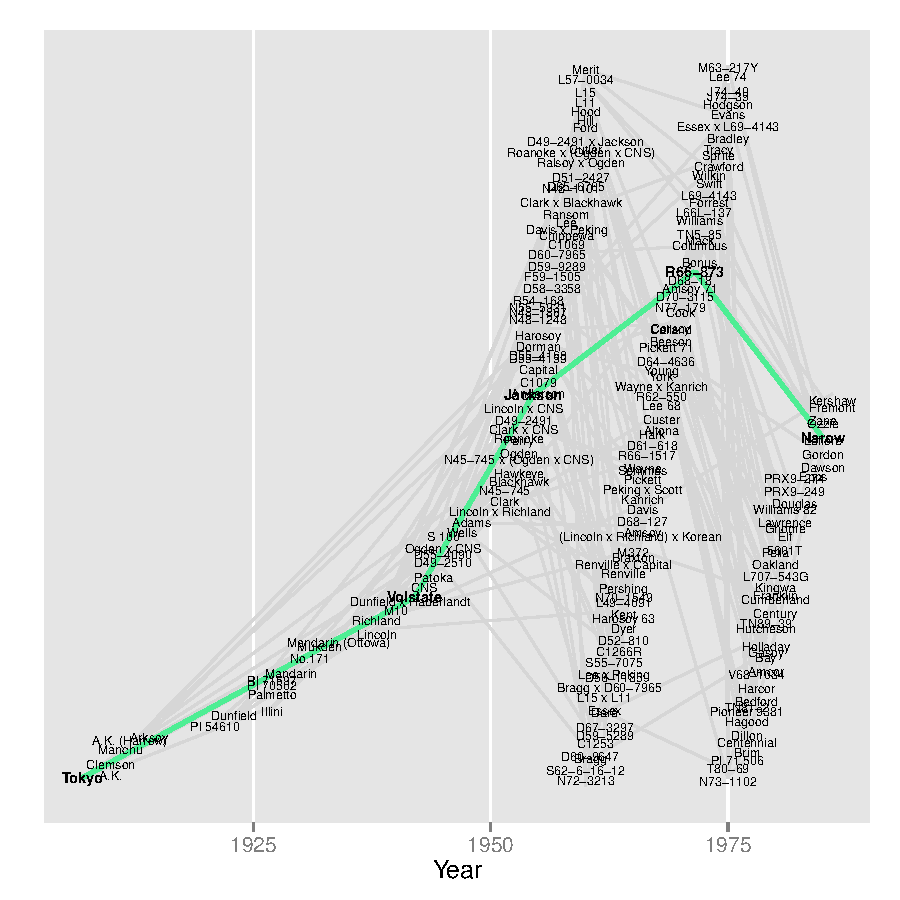
\includegraphics{ggenealogy-plotPathOnAll1}
\end{center} 
\caption{Plotting the path between Tokyo and Narow across full genealogical structure, using a binVector size of 3.}
\label{fig:plotPathOnAll1}
\end{figure}

While the first three explicit parameters to the function \texttt{plotPathOnAll()} have been introduced earlier in this paper, the fourth parameter (\texttt{binVector}) requires some explanation. The motivation of the \texttt{plotPathOnAll()} function is to write variety text labels on a plot, with the center of each variety label constricted on the horizontal axis to its developmental year. As is the case for the plots before, the vertical axis has no meaning other than pro- viding a plotting area in which to draw the text labels. Unfortunately, for large datasets, this motivation can be a difficult task because the text labels of the varieties can overlap if they are assigned a similar y coordinate, have a similar year (x coordinate), and have labels with large numbers of characters (width of x coordinate).

For each variety, the x coordinate (year) and width of the x coordinate (text label width) cannot be altered, as they provide useful information. However, for each variety, the vertical coordinate is arbitrary. Hence, in an attempt to mitigate text overlapping, the \texttt{plotPathOnAll()} function does not randomly assign the vertical coordinate. Instead, it allows users to partially control the vertical coordinates with a user-determined number of bins (\texttt{binVector}).

If the user determines to produce a plot using three bins, as in the example code above, then the varieties are all grouped into three bins based on their years of development. In other words, there will be bin 1 (the ``oldest bin") which includes one-third of the total number of varieties all with the oldest developmental years, bin 2 (the ``middle bin"), and bin 3 (the ``youngest bin").

Then, in order to decrease text overlap, the consecutively increasing vertical axis coordinates are alternatively assigned to the three bins (For example: bin 1, then bin 2, then bin 3, then bin 1, then bin 2, then bin 3, etc.) repeatedly until all varieties are accounted. This algorithm means that for any pair of varieties within a given bin constrained to those years on the horizontal axis, there are exactly two other varieties placed between them vertically on the vertical axis that come from the two other bins constrained to a different set of year values on the horizontal axis.

We see in the plot that edges not on the path of interest are thin and gray, whereas edges on the path of interest are bolded and green, by default. We also see that variety labels in the path of interest are boldfaced, by default.

The plot presents useful information: We immediately gather that the path of interest between ``Tokyo" and ``Narow" does span most of the years of the data structure. In fact, Tokyo appears to be the oldest variety present in the dataset, and Narow appears to be one of the youngest varieties. We can also determine that the vast majority of varieties appear to have development years between 1950 and 1970.

However, this plot has significant empty spaces between the noticeably distinct bins, whereas almost all text labels are overlapping, thereby decreasing their readability. To force some variety text labels into these spaces, the user may consider using a larger number of bins. Hence, we next examine a \texttt{binVector} size of six:

\begin{Schunk}
\begin{Sinput}
> plotPathOnAll(path, sbGeneal, ig, binVector = 1:6)
\end{Sinput}
\end{Schunk}

\setkeys{Gin}{width=6in, height=6in}
\begin{figure} 
  \begin{center} 
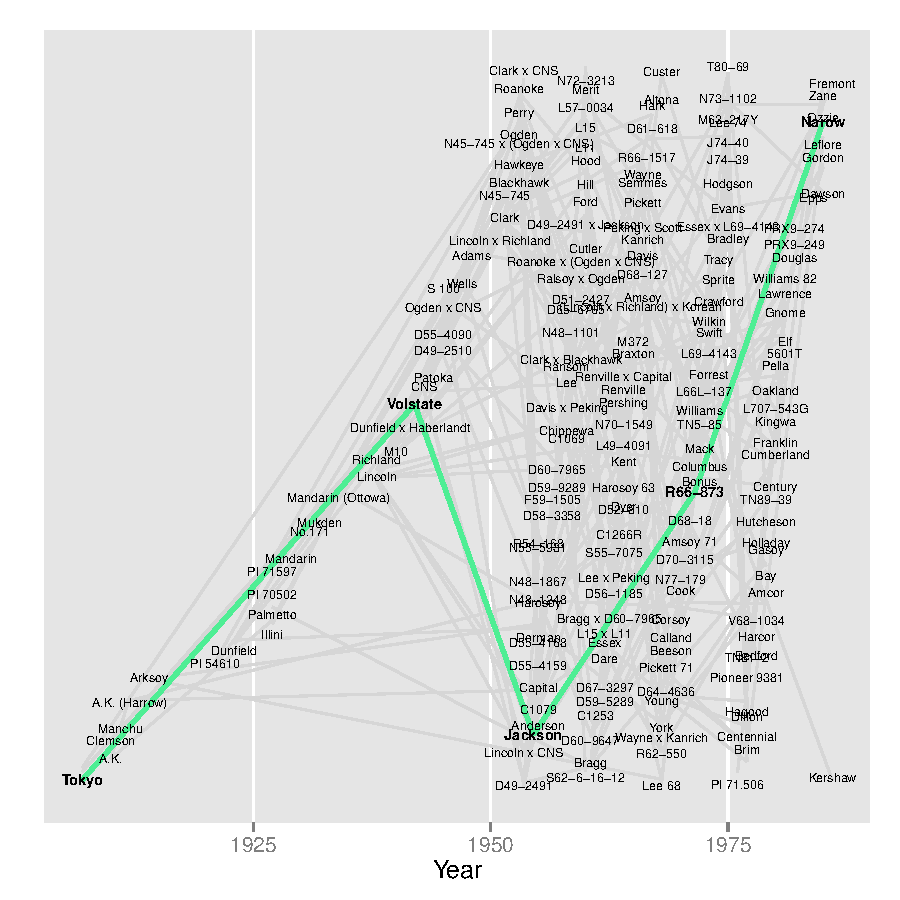
\includegraphics{ggenealogy-plotPathOnAll2}
\end{center} 
\caption{Plotting the path between Tokyo and Narow superimposed on the full genealogical structure, using a binVector size of six.}
\label{fig:plotPathOnAll2}
\end{figure}

We can immediately see that this plot more successfully mitigates text variety label overlap than the previous plot that had a \texttt{binVector} size of three. We can also confirm what we saw in the previous plot that indeed most varieties have development years between 1950 and 1970, and any remaining textual overlap is confined to this range of years.

\subsection{Plotting pairwise distance matrices between a set of vertices}

It may also be of interest to generate matrices where the colors indicates a variable (such as the degree of the shortest path) between all pairwise combinations of inputted varieties. The package \pkg{ggenealogy} also provides a function \texttt{plotDegMatrix()} for that purpose.

Here we generate a distance matrix for a set of 8 varieties, defining the x-axis title and y-axis title as ``Soybean label", and the legend label as ``Degree". Syntax from the \texttt{ggplot2} package can be appended to tailor the output from the \texttt{plotDegMatrix()} function. In this case, we specify that pairs with small degrees are colored white, while pairs with large degrees are colored dark green:

\begin{Schunk}
\begin{Sinput}
> varieties=c("Brim", "Bedford", "Calland", "Narow", "Pella", "Tokyo", "Young", "Zane")
> p = plotDegMatrix(varieties, ig, sbGeneal, "Soybean label", "Soybean label", "Degree")
> p + ggplot2::scale_fill_continuous(low="white", high="darkgreen")
\end{Sinput}
\end{Schunk}

\setkeys{Gin}{width=6in, height=6in}
\begin{figure} 
  \begin{center} 
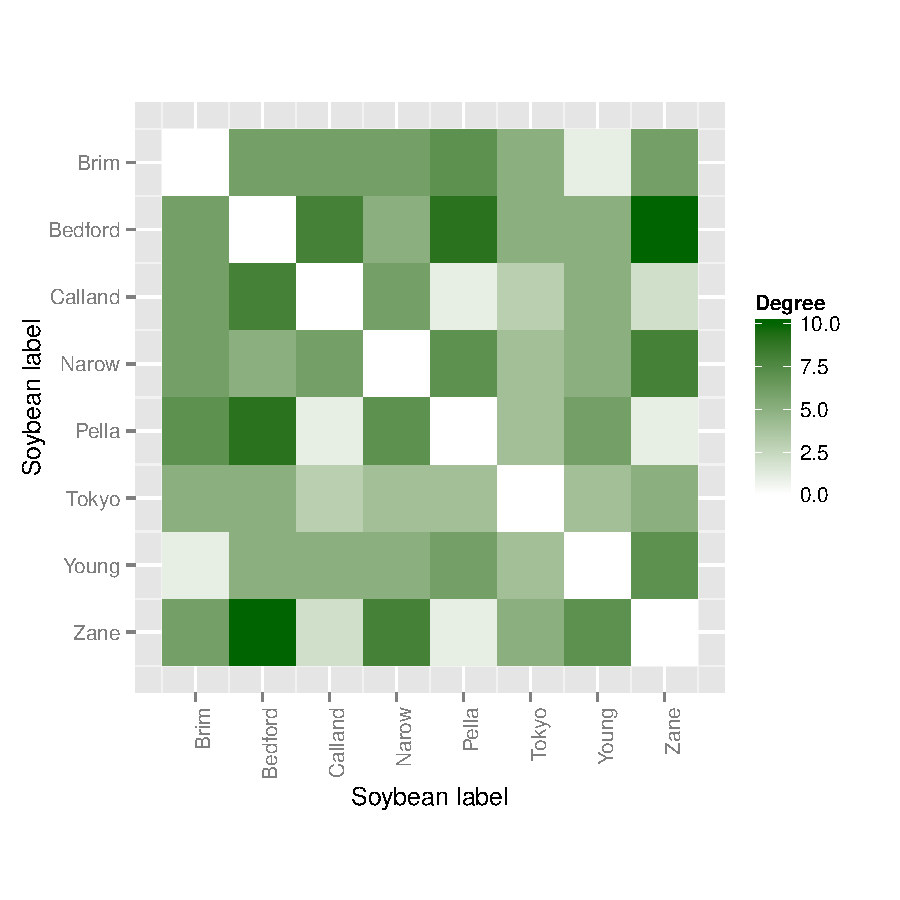
\includegraphics{ggenealogy-plotDegMatrix1}
\end{center} 
\caption{Plotting the degree matrix between eight varieties of interest.}
\label{fig:plotDegMatrix1}
\end{figure}

We see that the degree of the shortest path between varieties ``Bedford" and ``Zane" seems to be the largest in the dataset, which should be around 10. We can verify this simply with:

\begin{Schunk}
\begin{Sinput}
> getDegree("Bedford", "Zane", ig, sbGeneal)
\end{Sinput}
\begin{Soutput}
[1] 10
\end{Soutput}
\end{Schunk}

Indeed, the degree of the shortest path between ``Bedford" and ``Zane" is 10. However, what the distance matrix additionally tells us is that a degree of 10 may be a comparatively large degree for this given soybean dataset, at least in that the degrees of the shortest paths for the other 27 pairwise combinations of varieties that we explored here are less than 10.

In a similar function, \texttt{plotYearMatrix()}, the difference in years between all pairwise combinations of vertices can be constructed and viewed:

\begin{Schunk}
\begin{Sinput}
> varieties=c("Brim", "Bedford", "Calland", "Narow", "Pella", "Tokyo", "Young", "Zane")
> plotYearMatrix(varieties,sbGeneal)
\end{Sinput}
\end{Schunk}

\setkeys{Gin}{width=6in, height=6in}
\begin{figure} 
  \begin{center} 
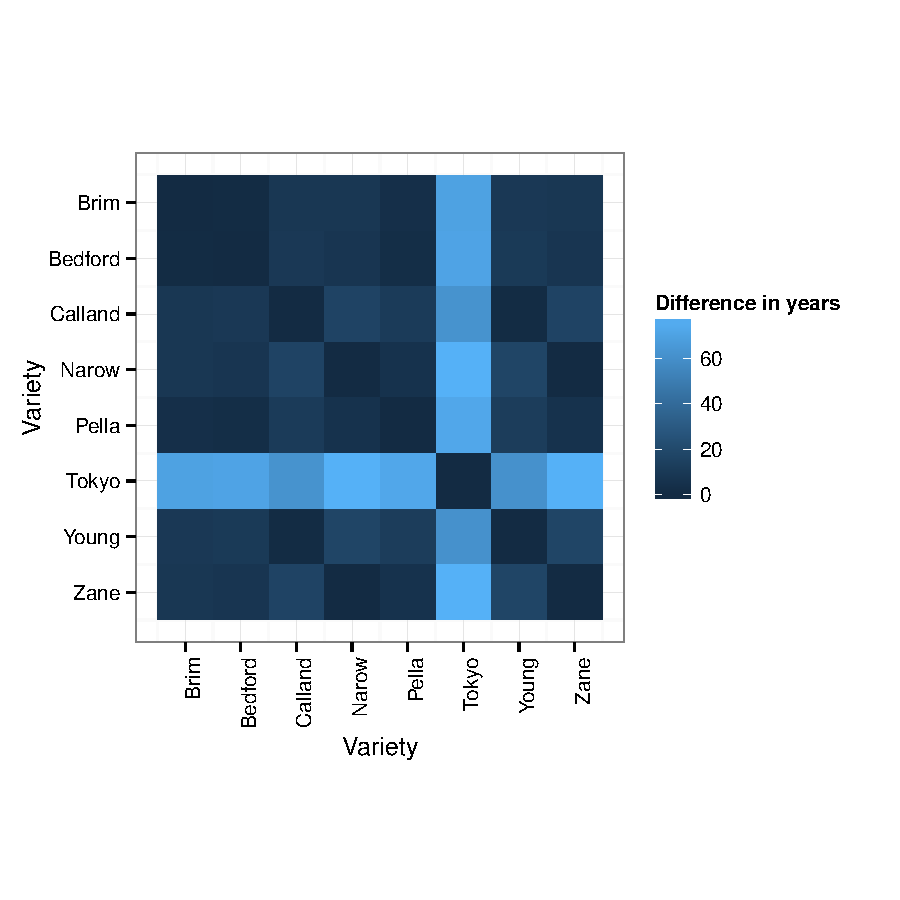
\includegraphics{ggenealogy-plotYearMatrix1}
\end{center} 
\caption{Ancestors and Descendants of tree.}
\label{fig:plotYearMatrix1}
\end{figure}

Here, we did not change any defaults. As such, the x-axis and y-axis labels are the default value ``Variety", the legend key label is the default value ``Difference in years", and the default color of the matrix is dark blue for small year difference and light blue for large year difference.

Running this function on this particular set of vertices shows that most combinations of varieties are only one or two decades apart in year introduction, with the exception of the ``Tokyo" variety, which appears to be separated from each of the other seven varities by about six decades. This should not be too surprising, because we have seen througout the tutorial that the ``Tokyo" variety is the oldest variety in the dataset.

\section{Conclusions}

The \pkg{ggenealogy} package offers various plotting tools that can assist those studying genealogical lineages in the data exploration phases. As each plot comes with its pros and cons, we recommend for users to explore several of the available visualization tools.

This vignette briefly introduced some of the capabilities of the \pkg{ggenealogy} package. Inevitably, new applications will demand new features in subsequent versions and might reveal unforeseen bugs. Please send comments or suggestions and report bugs to \texttt{lrutter@iastate.edu}.

\end{document}
